\documentclass[journal,12pt,twocolumn]{IEEEtran}
%
\usepackage{setspace}
\usepackage{gensymb}
\usepackage{xcolor}
\usepackage{caption}
%\usepackage{subcaption}
%\doublespacing
\singlespacing
\usepackage{multicol}
%\usepackage{eenrc}
\usepackage{iithtlc}
%\usepackage{graphicx}
%\usepackage{amssymb}
%\usepackage{relsize}
\usepackage[cmex10]{amsmath}
\usepackage{mathtools}
%\usepackage{amsthm}
%\interdisplaylinepenalty=2500
%\savesymbol{iint}
%\usepackage{txfonts}
%\restoresymbol{TXF}{iint}
%\usepackage{wasysym}
\usepackage{amsthm}
\usepackage{mathrsfs}
\usepackage{txfonts}
\usepackage{stfloats}
\usepackage{cite}
\usepackage{cases}
\usepackage{subfig}
%\usepackage{xtab}
\usepackage{longtable}
\usepackage{multirow}
%\usepackage{algorithm}
%\usepackage{algpseudocode}
\usepackage{enumitem}
\usepackage{mathtools}
%\usepackage{stmaryrd}
\usepackage{graphicx}
\usepackage{listings}
\usepackage{circuitikz}
    \usepackage[latin1]{inputenc}                                 %%
    \usepackage{color}                                            %%
    \usepackage{array}                                            %%
    \usepackage{longtable}                                        %%
    \usepackage{calc}                                             %%
    \usepackage{multirow}                                         %%
    \usepackage{hhline}                                           %%
    \usepackage{ifthen}                                           %%
  %optionally (for landscape tables embedded in another document): %%
    \usepackage{lscape}     
\usepackage{url}
\def\UrlBreaks{\do\/\do-}

%\usepackage{wasysym}
%\newcounter{MYtempeqncnt}
\DeclareMathOperator*{\Res}{Res}
%\renewcommand{\baselinestretch}{2}
\renewcommand\thesection{\arabic{section}}
\renewcommand\thesubsection{\thesection.\arabic{subsection}}
\renewcommand\thesubsubsection{\thesubsection.\arabic{subsubsection}}

\renewcommand\thesectiondis{\arabic{section}}
\renewcommand\thesubsectiondis{\thesectiondis.\arabic{subsection}}
\renewcommand\thesubsubsectiondis{\thesubsectiondis.\arabic{subsubsection}}

% correct bad hyphenation here
\hyphenation{op-tical net-works semi-conduc-tor}

\def\inputGnumericTable{}  

\lstset{
language=python,
frame=single, 
breaklines=true
}

\begin{document}
%

\theoremstyle{definition}

\newtheorem{theorem}{Theorem}[section]
\newtheorem{problem}{Problem}
\newtheorem{proposition}{Proposition}[section]
\newtheorem{lemma}{Lemma}[section]
\newtheorem{corollary}[theorem]{Corollary}
\newtheorem{example}{Example}[section]
\newtheorem{definition}{Definition}[section]
%\newtheorem{algorithm}{Algorithm}[section]
%\newtheorem{cor}{Corollary}
\newcommand{\BEQA}{\begin{eqnarray}}
\newcommand{\EEQA}{\end{eqnarray}}
\newcommand{\define}{\stackrel{\triangle}{=}}

\bibliographystyle{IEEEtran}
%\bibliographystyle{ieeetr}



\providecommand{\pr}[1]{\ensuremath{\Pr\left(#1\right)}}
\providecommand{\qfunc}[1]{\ensuremath{Q\left(#1\right)}}
\providecommand{\sbrak}[1]{\ensuremath{{}\left[#1\right]}}
\providecommand{\lsbrak}[1]{\ensuremath{{}\left[#1\right.}}
\providecommand{\rsbrak}[1]{\ensuremath{{}\left.#1\right]}}
\providecommand{\brak}[1]{\ensuremath{\left(#1\right)}}
\providecommand{\lbrak}[1]{\ensuremath{\left(#1\right.}}
\providecommand{\rbrak}[1]{\ensuremath{\left.#1\right)}}
\providecommand{\cbrak}[1]{\ensuremath{\left\{#1\right\}}}
\providecommand{\lcbrak}[1]{\ensuremath{\left\{#1\right.}}
\providecommand{\rcbrak}[1]{\ensuremath{\left.#1\right\}}}
\theoremstyle{remark}
\newtheorem{rem}{Remark}
\newcommand{\sgn}{\mathop{\mathrm{sgn}}}
\providecommand{\abs}[1]{\left\vert#1\right\vert}
\providecommand{\res}[1]{\Res\displaylimits_{#1}} 
\providecommand{\norm}[1]{\lVert#1\rVert}
\providecommand{\mtx}[1]{\mathbf{#1}}
\providecommand{\mean}[1]{E\left[ #1 \right]}
\providecommand{\fourier}{\overset{\mathcal{F}}{ \rightleftharpoons}}
%\providecommand{\hilbert}{\overset{\mathcal{H}}{ \rightleftharpoons}}
\providecommand{\system}{\overset{\mathcal{H}}{ \longleftrightarrow}}
\providecommand{\gauss}[2]{\mathcal{N}\ensuremath{\left(#1,#2\right)}}
	%\newcommand{\solution}[2]{\textbf{Solution:}{#1}}
\newcommand{\solution}{\noindent \textbf{Solution: }}
\providecommand{\dec}[2]{\ensuremath{\overset{#1}{\underset{#2}{\gtrless}}}}
%\numberwithin{equation}{section}
%\numberwithin{problem}{section}

\def\putbox#1#2#3{\makebox[0in][l]{\makebox[#1][l]{}\raisebox{\baselineskip}[0in][0in]{\raisebox{#2}[0in][0in]{#3}}}}
     \def\rightbox#1{\makebox[0in][r]{#1}}
     \def\centbox#1{\makebox[0in]{#1}}
     \def\topbox#1{\raisebox{-\baselineskip}[0in][0in]{#1}}
     \def\midbox#1{\raisebox{-0.5\baselineskip}[0in][0in]{#1}}


% paper title
% can use linebreaks \\ within to get better formatting as desired

%\title{FM Signal Transmission Using Pi}
 
 
%\title{Electrical Circuit Design using Latex}

\title{\logo{Amplitude Phase Shift Keying}} 
 
%
%
% author names and IEEE memberships
% note positions of commas and nonbreaking spaces ( ~ ) LaTeX will not break
% a structure at a ~ so this keeps an author's name from being broken across
% two lines.
% use \thanks{} to gain access to the first footnote area
% a separate \thanks must be used for each paragraph as LaTeX2e's \thanks
% was not built to handle multiple paragraphs
%

%\author{Y Aditya, A Rathnakar and G V V Sharma$^{*}$% <-this % stops a space
%\author{K Prasanna Kumar  %<-this  stops a space
%\thanks{The author is Project Associate in National Resource Centre - IIT Hyderabad
%502285 India e-mail: kk.prassu924@gmail.com 
%}}

\author{K Prasanna Kumar %<-this  stops a space
\thanks{Author is from dept. of Electrical Engineering IIT Hyderabad, Email: kprasannakumar@iith.ac.in}}


% make the title area
\maketitle


\tableofcontents

\bigskip

\begin{abstract}
This module explains about the comparative study of M-array Phase Shift keying and M-array Amplitude Phase Shift Keying.
\end{abstract}
\section{QPSK}
\begin{figure}[h!]
\centering
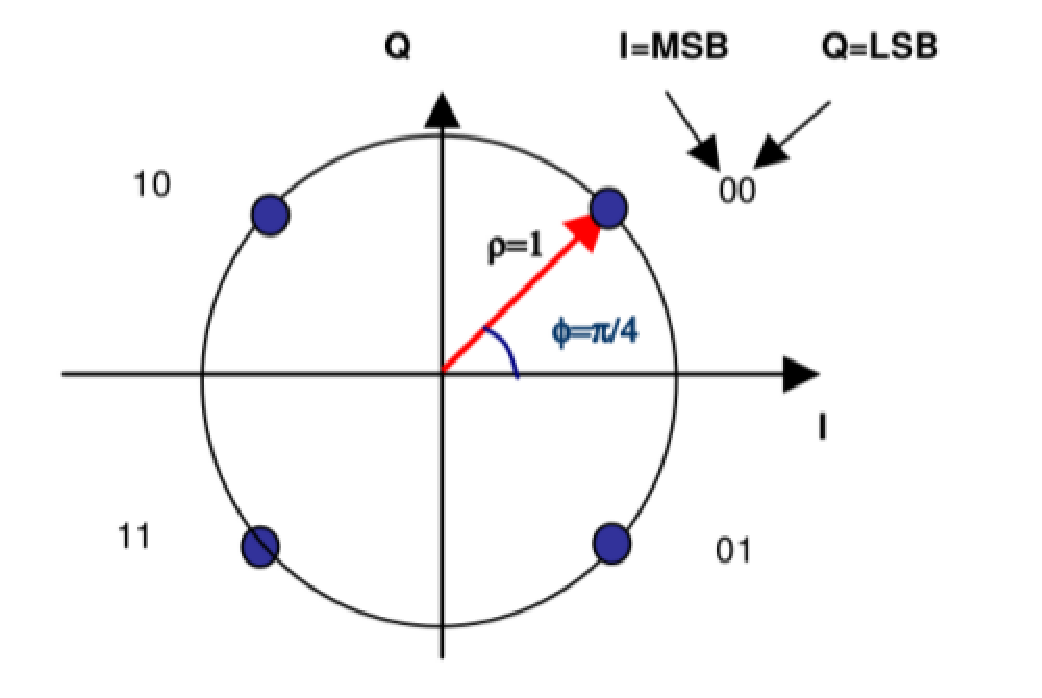
\includegraphics[scale=0.4]{figs/qpsk_con}
\label{QPSK Constellation Diagram}
\caption{QPSK Constellation Diagram}
\end{figure}
$$X =Re^{i\theta} = Rcos(\theta) + iRsin(\theta)$$ 
Where R and $\theta$ depends upon the positon of the constalation symbol accounding polar coordinate System.
$$N = A + iB $$
Here, N is the complex AWGN noise and A, B are random variable.
$$ Y = X + N =(Rcos\theta + A) + i (Rsin\theta + B) $$
Y is the received signal from the channel.  
\begin{lstlisting}
wget https://raw.githubusercontent.com/PrasannaIITH/APSK/master/codes/QPSK.py
\end{lstlisting}
\section{8PSK}
\begin{figure}[h!]
\centering
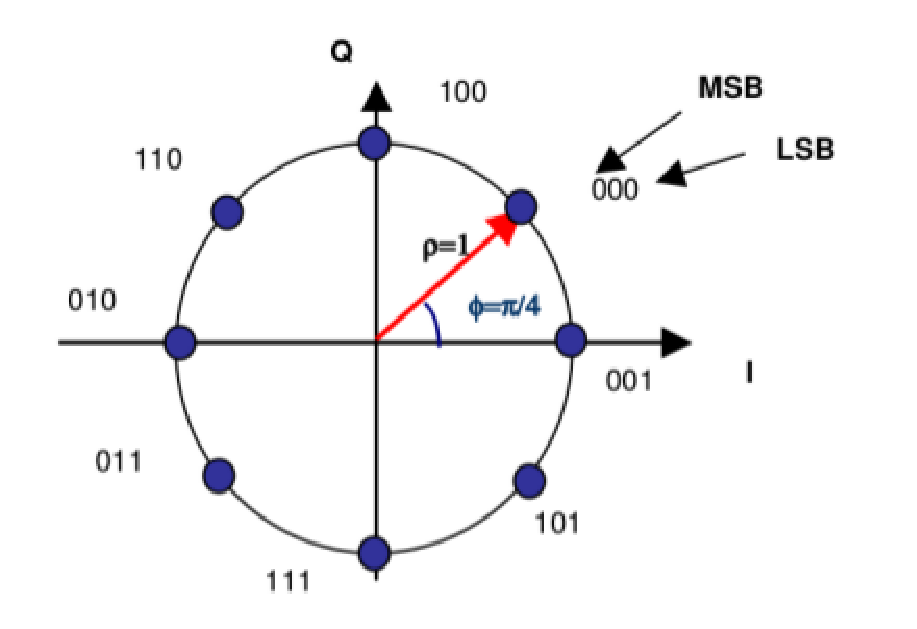
\includegraphics[scale=0.4]{figs/8PSK_CON.eps}
\label{8PSK Constellation Diagram}
\caption{8PSK Constellation Diagram}
\end{figure}
\begin{lstlisting}
wget https://raw.githubusercontent.com/PrasannaIITH/APSK/master/codes/8PSK.py
\end{lstlisting}


\section{16APSK}
\begin{figure}[h!]
\centering
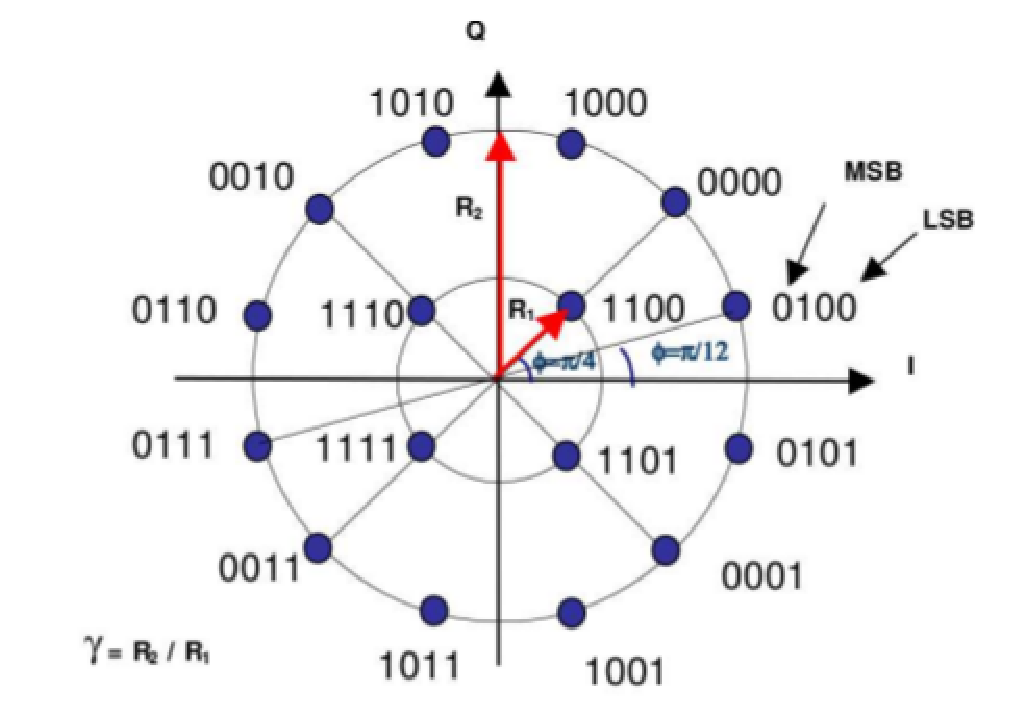
\includegraphics[scale=0.4]{figs/16APSK.eps}
\label{16APSK Constellation Diagram}
\caption{16APSK Constellation Diagram}
\end{figure}

\begin{lstlisting}
wget https://raw.githubusercontent.com/PrasannaIITH/APSK/master/codes/16APSK.py
\end{lstlisting}
\section{32APSK}
\begin{figure}[h!]
\centering
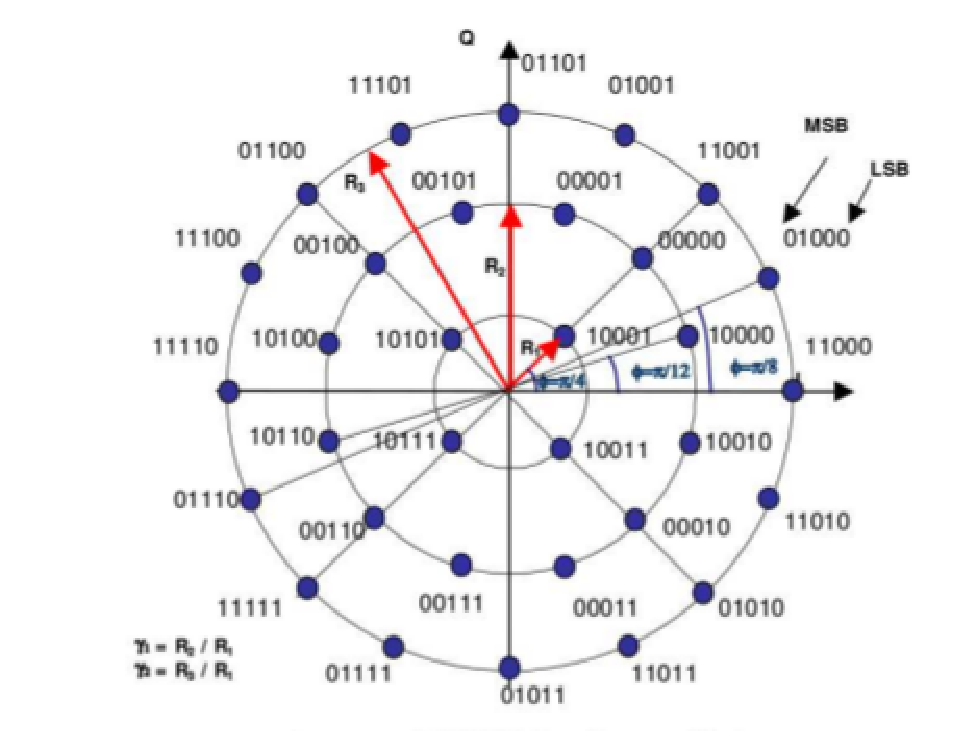
\includegraphics[scale=0.4]{figs/32APSK.eps}
\label{32APSK Constellation Diagram}
\caption{32APSK Constellation Diagram}
\end{figure}
%
%\begin{thebibliography}{00}
%\bibitem{b1} xxxxxxx, xxxxxxxxxxxxxx url{http://www.wiringpi.com/}. 
%\bibitem{b2} Sunfounder,xxxxxxxxxxxxxxxx \url{https://www.youtube.com/watch?time_continue=4&v=y3Pv7--6eik}.
%\end{thebibliography}
\end{document}
